
\section{Inequalities}
\begin{itemize}
\item[1.] $\ln x\leq x-1$
\item[2.] Convex function
<1>. $f(x)$ is convex $\Leftrightarrow \forall x_1,x_2,\lambda\in[0,1]$, $$f\left(\lambda x_1+(1-\lambda)x_2\right)\leq\lambda f(x_1)+(1-\lambda)f(x_2)$$
<2>. $f''(x)\geq 0\Rightarrow f(x)$ is convex.\\
proof: From Taylor's Theorem, $f''(x)\geq 0$:
$$f(y) \geq f(x) + f'(x)(y-x)$$
Let $z = \lambda x + (1-\lambda)y$:
\begin{align*}
1.\ f(x) &\geq f(z) + f'(z)(x-z) \\
2.\ f(y) &\geq f(z) + f'(z)(y-z) \\
\lambda\cdot 1. + (1-\lambda)\cdot 2. \Rightarrow \lambda f(x) + (1-\lambda)f(y) &\geq f(z) + f'(z)(\lambda x + (1-\lambda)y - z) \\
&= f(z) = f(\lambda x + (1-\lambda)y)
\end{align*}
So $f(x)$ is convex.

\item[3.] Jensen's Inequality
$$\mathbb{E}\left[f(X)\right]\geq f\left[\mathbb{E}(X)\right]$$

\item[4.] Sum-log Inequality(求和不等式)
$\forall a_1,\cdots,a_n,b_1,\cdots,b_n>0$:
$$\sum_{i=1}^{n}a_i\log\dfrac{a_i}{b_i}\geq \left(\sum_{i=1}^{n}a_i\right)\log\dfrac{\sum\limits_{i=1}^{n}a_i}{\sum\limits_{i=1}^{n}b_i}$$
With equality if and only if $a_i=\lambda b_i$ for all $i$, \textcolor{red}{with same $\lambda$}.\\
Specifically, when $n=2$:
$$a_1\log\dfrac{a_1}{b_1}+a_2\log\dfrac{a_2}{b_2}\geq (a_1+a_2)\log\dfrac{a_1+a_2}{b_1+b_2}$$
proof:\ Let $f(t)=t\log t$, then $f''(t)=\dfrac{1}{t}\geq 0$.
Let $p_i=\dfrac{b_i}{\sum\limits_{i=1}^{n}b_i}$,$t_i=\dfrac{a_i}{b_i}$.
\begin{align*}
\sum_{i=1}^np_if(t_i) &\geq f\left(\sum_{i=1}^np_it_i\right) \\
\sum_{i=1}^n\left[\dfrac{\textcolor{blue}{b_i}}{\sum\limits_{j=1}^{n}b_j}\left(\dfrac{a_i}{\textcolor{blue}{b_i}}\log\dfrac{a_i}{b_i}\right)\right] &\geq \left[\sum_{i=1}^n\left(\dfrac{\textcolor{blue}{b_i}}{\sum\limits_{j=1}^{n}b_j}\cdot\dfrac{a_i}{\textcolor{blue}{b_i}}\right)\right]\log\left[\sum_{i=1}^n\left(\dfrac{\textcolor{blue}{b_i}}{\sum\limits_{j=1}^{n}b_j}\cdot\dfrac{a_i}{\textcolor{blue}{b_i}}\right)\right] \\
\dfrac{1}{\textcolor{blue}{\sum\limits_{j=1}^{n}b_j}}\cdot \sum_{i=1}^na_i\log\dfrac{a_i}{b_i} &\geq \dfrac{1}{\textcolor{blue}{\sum\limits_{j=1}^{n}b_j}}\cdot \left(\sum_{i=1}^{n}a_i\right)\log\dfrac{\sum\limits_{i=1}^{n}a_i}{\sum\limits_{i=1}^{n}b_i} \\
\sum_{i=1}^na_i\log\dfrac{a_i}{b_i} &\geq \left(\sum_{i=1}^{n}a_i\right)\log\dfrac{\sum\limits_{i=1}^{n}a_i}{\sum\limits_{i=1}^{n}b_i} \\
\end{align*}
\end{itemize}

\newpage

\begin{proposition}
$H(\vec{p})$ is concave in $\vec{p}$.\\
$\forall \vec{p}_1,\vec{p}_2,\lambda\in[0,1]$:
\begin{align*}
H(\lambda\vec{p}_1+(1-\lambda)\vec{p}_2) &= -\sum_{x\in \mathcal{X}}\left[\lambda p_1(x)+(1-\lambda)p_2(x)\right]\log\left[\lambda p_1(x)+(1-\lambda)p_2(x)\right] \\
&= -\sum_{x\in \mathcal{X}}\left[\textcolor{red}{\lambda p_1(x)}+\textcolor{blue}{(1-\lambda)p_2(x)}\right]\log\dfrac{\textcolor{red}{\lambda p_1(x)}+\textcolor{blue}{(1-\lambda)p_2(x)}}{\textcolor{yellow}{\lambda} + \textcolor{green}{(1-\lambda)}} \\
&= -\sum_{x\in \mathcal{X}}\left[\textcolor{red}{a_1(x)}+\textcolor{blue}{a_2(x)}\right]\log\dfrac{\textcolor{red}{a_1(x)}+\textcolor{blue}{a_2(x)}}{\textcolor{yellow}{b_1} + \textcolor{green}{b_2}}
\end{align*}
Where $a_1(x)=\lambda p_1(x)$, $a_2(x)=(1-\lambda)p_2(x)$, $b_1=\lambda$, $b_2=1-\lambda$, since $a_1(x),b_1,a_2(x),b_2>0$, and the log-sum Inequality:
$$a_1\log\dfrac{a_1}{b_1}+a_2\log\dfrac{a_2}{b_2}\geq (a_1+a_2)\log\dfrac{a_1+a_2}{b_1+b_2}$$
So
$$\left[a_1(x)+a_2(x)\right]\log\dfrac{a_1(x)+a_2(x)}{b_1 + b_2}\leq a_1(x)\log\dfrac{a_1(x)}{b_1}+a_2(x)\log\dfrac{a_2(x)}{b_2}$$
i.e.
\begin{align*}
H(\lambda\vec{p}_1+(1-\lambda)\vec{p}_2) &\geq -\sum_{x\in\mathcal{X}} \left[\lambda p_1(x)\log\dfrac{\lambda p_1(x)}{\lambda} + (1-\lambda)p_2(x)\log\dfrac{(1-\lambda)p_2(x)}{1-\lambda}\right] \\
&= \lambda \left(-\sum_{x\in\mathcal{X}} p_1(x)\log p_1(x)\right) + (1-\lambda)\left(-\sum_{x\in\mathcal{X}} p_2(x)\log p_2(x)\right) \\
&= \lambda H(\vec{p}_1) + (1-\lambda)H(\vec{p}_2)
\end{align*}
So $H(\vec{p})$ is concave in $\vec{p}$.
\end{proposition}

\begin{proposition}
\begin{itemize}
\item[1.] $I(X;Y)$ is \textcolor{red}{the function of $p(x,y)$}, but it is non-convex and non-concave in $p(x,y)$.
\item[2.] If $p(y|x)$ is fixed(given), $I(X;Y)$ is concave in $p(x)$.
\item[3.] $X\sim p(x)$, $H(X)$ is concave in $p(x)$.
\item[4.] If $p(x)$ is fixed(given), $I(X;Y)$ is convex in $p(y|x)$.
\end{itemize}

Lemma: If $f(x)$ is convex, $g(x)$ is an increasing linear function, then $f(g(x))$ is convex.

\end{proposition}

2. If $p(y|x)$ is fixed(given), $I(X;Y)$ is concave in $p(x)$.\\
proof:
\begin{align*}
I(X;Y) &= H(Y) - H(Y|X) \\
&= \sum_{y}\underbrace{p(y)\log\dfrac{1}{p(y)}}_{x\log x \text{\ is convex}} - \underbrace{\sum_{x}p(x)H(Y|X=x)}_{\text{linear to } p(x)}
\end{align*}
由于$p(y)=\sum\limits_{x}p(x)p(y|x)$, 所以$p(y)$是关于$p(x)$的线性函数, 所以$H(Y)$关于$p(y)$是concave, 关于$p(x)$也是concave的. \\
So $I(X;Y)$ is concave in $p(x)$.

3. $X\sim p(x)$, $H(X)$ is concave in $p(x)$. \\
Define $\Theta$: Time sharing random variable. \\
$$\Theta=\left\{\begin{array}{l}1, \text{\ \ \ w.p.\ \ } \lambda \\2, \text{\ \ \ w.p.\ \ } 1-\lambda\end{array}\right.$$
Let $Z=X_{\Theta}$, where $X_1\sim p_1(x)$, $X_2\sim p_2(x)$, so $Z\sim \lambda p_1(x)+(1-\lambda)p_2(x)$.
And since that $H(Z)\geq H(Z|\Theta)$, so we have
\begin{align*}
H(Z) &\geq H(Z|\Theta) \\
&= p(\Theta=1)H(Z|\Theta=1)+p(\Theta=2)H(Z|\Theta=2) \\
&= \lambda H(X_1) + (1-\lambda)H(X_2)
\end{align*}
i.e. $$H(p_{\lambda})\geq \lambda H(p_1) + (1-\lambda)H(p_2)$$
So $H(X)$ is concave in $p(x)$.

4. If $p(x)$ is fixed(given), $I(X;Y)$ is convex in $p(y|x)$. \\
define: $3$个概率分布: $p_1(y|x), p_2(y|x), p_{\lambda}(y|x)$, where \\
$p_{\lambda}(y|x)=\lambda p_1(y|x)+(1-\lambda)p_2(y|x)$, $p_1(x)=p_2(x)=p_{\lambda}(x)=p(x)$.
So
\begin{align*}
I_i(X;Y) &= \sum_{x,y}p_i(x,y)\log\dfrac{p_i(x,y)}{p_i(x)p_i(y)},\ \  i=1,2 \\
I_{\lambda}(X;Y) &= \sum_{x,y}p_{\lambda}(x,y)\log\dfrac{p_{\lambda}(x,y)}{p_{\lambda}(x)p_{\lambda}(y)}
\end{align*}
From log-sum Inequality with $n=2$:
$$(a_1+a_2)\log\dfrac{a_1+a_2}{b_1+b_2}\leq a_1\log\dfrac{a_1}{b_1}+a_2\log\dfrac{a_2}{b_2}$$
\begin{align*}
I_{\lambda}(X;Y) &= \sum_{x,y}p_{\lambda}(x,y)\log\dfrac{p_{\lambda}(x,y)}{p_{\lambda}(x)p_{\lambda}(y)} \\
&= \sum_{x,y}p_{\lambda}(y|x)p_{\lambda}(x)\log\dfrac{p_{\lambda}(y|x)}{p_{\lambda}(y)} \\
&= \sum_{x}p(x)\sum_y\left(\underbrace{\textcolor{blue}{\lambda p_1(y|x)}}_{\textcolor{blue}{a_1}}+\underbrace{\textcolor{red}{(1-\lambda)p_2(y|x)}}_{\textcolor{red}{a_2}}\right)\log\dfrac{\textcolor{blue}{\lambda p_1(y|x)}+\textcolor{red}{(1-\lambda)p_2(y|x)}}{\underbrace{\textcolor{green}{\lambda p_1(y)}}_{\textcolor{green}{b_1}}+\underbrace{\textcolor{yellow}{(1-\lambda)p_2(y)}}_{\textcolor{yellow}{b_2}}} \\
&\leq \sum_{x}p(x)\sum_y\left[\lambda p_1(y|x)\log\dfrac{\lambda p_1(y|x)}{\lambda p_1(y)}+(1-\lambda)p_2(y|x)\log\dfrac{(1-\lambda)p_2(y|x)}{(1-\lambda)p_2(y)}\right] \\
&= \lambda\sum_{x}p(x)\sum_y p_1(y|x)\log\dfrac{p_1(y|x)}{p_1(y)} + (1-\lambda)\sum_{x}p(x)\sum_y p_2(y|x)\log\dfrac{p_2(y|x)}{p_2(y)} \\
&= \lambda I_1(X;Y) + (1-\lambda)I_2(X;Y)
\end{align*}
So we have proved that $I(X;Y)$ is convex in $p(y|x)$.\\

\begin{proposition}
Markov Chain: $X\rightarrow Y\rightarrow Z$, 看作是双向的, i.e. 这等价于 $X\leftrightarrow Y\leftrightarrow Z$.\\
$$X\perp Z|Y$$
$$p(x,y,z)=p(x)p(y|x)p(z|y)\Leftrightarrow p(z|xy)=p(z|y)$$
$$H(Z|XY)=H(Z|Y)$$
\end{proposition}

\begin{proposition}
Independent $\nRightarrow$ Conditional Independent.
$$X\perp Y; X\not\perp Y|Z$$
\begin{figure}[htbp]
    \centering
    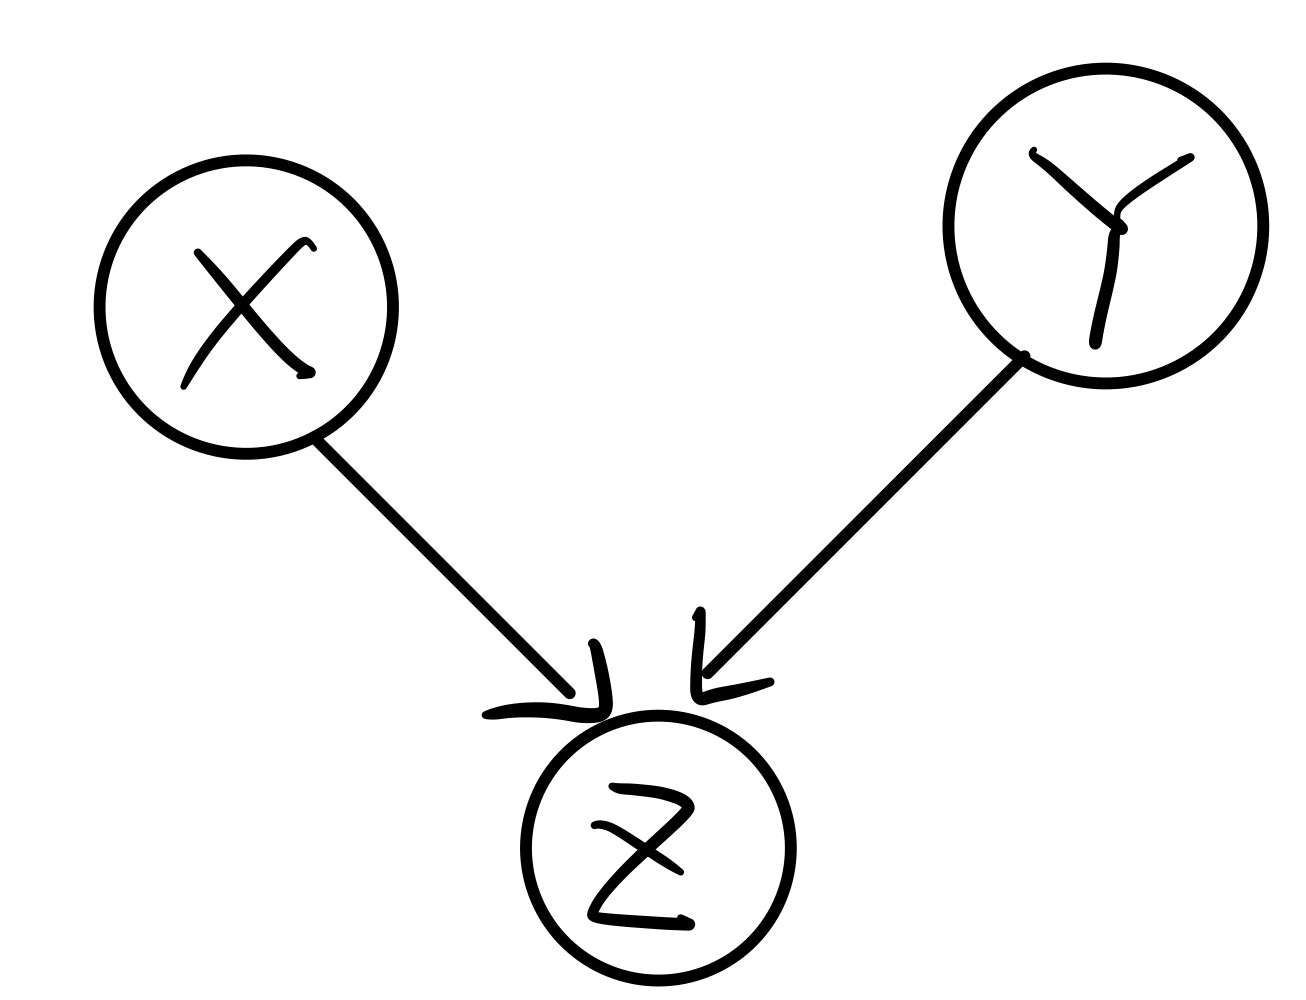
\includegraphics[width=0.5\textwidth]{./figures/chapter1/conditional_independent.png}
\end{figure}
\end{proposition}

\begin{proposition}
\textcolor{red}{If $Z=g(Y)$, then $X\rightarrow Y\rightarrow Z$}.
\end{proposition}

\begin{proposition}
Data Processing Inequality(数据处理不等式): For a Markov Chain $$X\rightarrow Y\rightarrow Z, I(X;Y)\geq I(X;Z)$$
$$X\rightarrow Y\rightarrow Z\rightarrow M, I(X;M)\leq I(Y;Z)$$
物理意义: 数据在不断处理的过程中, 相关性不断下降. \\
\textcolor{red}{处理后的相关性 $\leq$ 处理前的相关性.} \\
传递信息的过程中, 最好的情况是信息量不减少, 后面的数据不会有办法与更往前的数据有更强的相关性. \\
proof:
\begin{align*}
I(X;Y,Z) &= I(X;Y) + I(X;Z|Y) \\
&= I(X;Z) + I(X;Y|Z)
\end{align*}
Since $I(X;Z|Y)=0$, so $I(X;Y)=I(X;Z)+I(X;Y|Z)\geq I(X;Z)$.
i.e. $$I(X;Y)\geq I(X;Z)$$
\end{proposition}

\begin{proposition}
With Markov Chain $X\rightarrow Y\rightarrow Z$
$$I(X;Y)\geq I(X;Y|Z)$$
In general, 这两个互信息无法进行比较, 但是\textcolor{red}{满足以上Markov Chain时成立!}

由上个定理的证明: $I(X;Y)=I(X;Z)+I(X;Y|Z)$, 由于$I(X;Z)\geq 0$:
$$I(X;Y)\geq I(X;Y|Z)$$

物理意义: $X,Z$的互信息不能完全表达出$X,Y$的互信息, 剩余的部分由$X,Y|Z$的互信息来表达.

\end{proposition}

\begin{figure}[htbp]
    \centering
    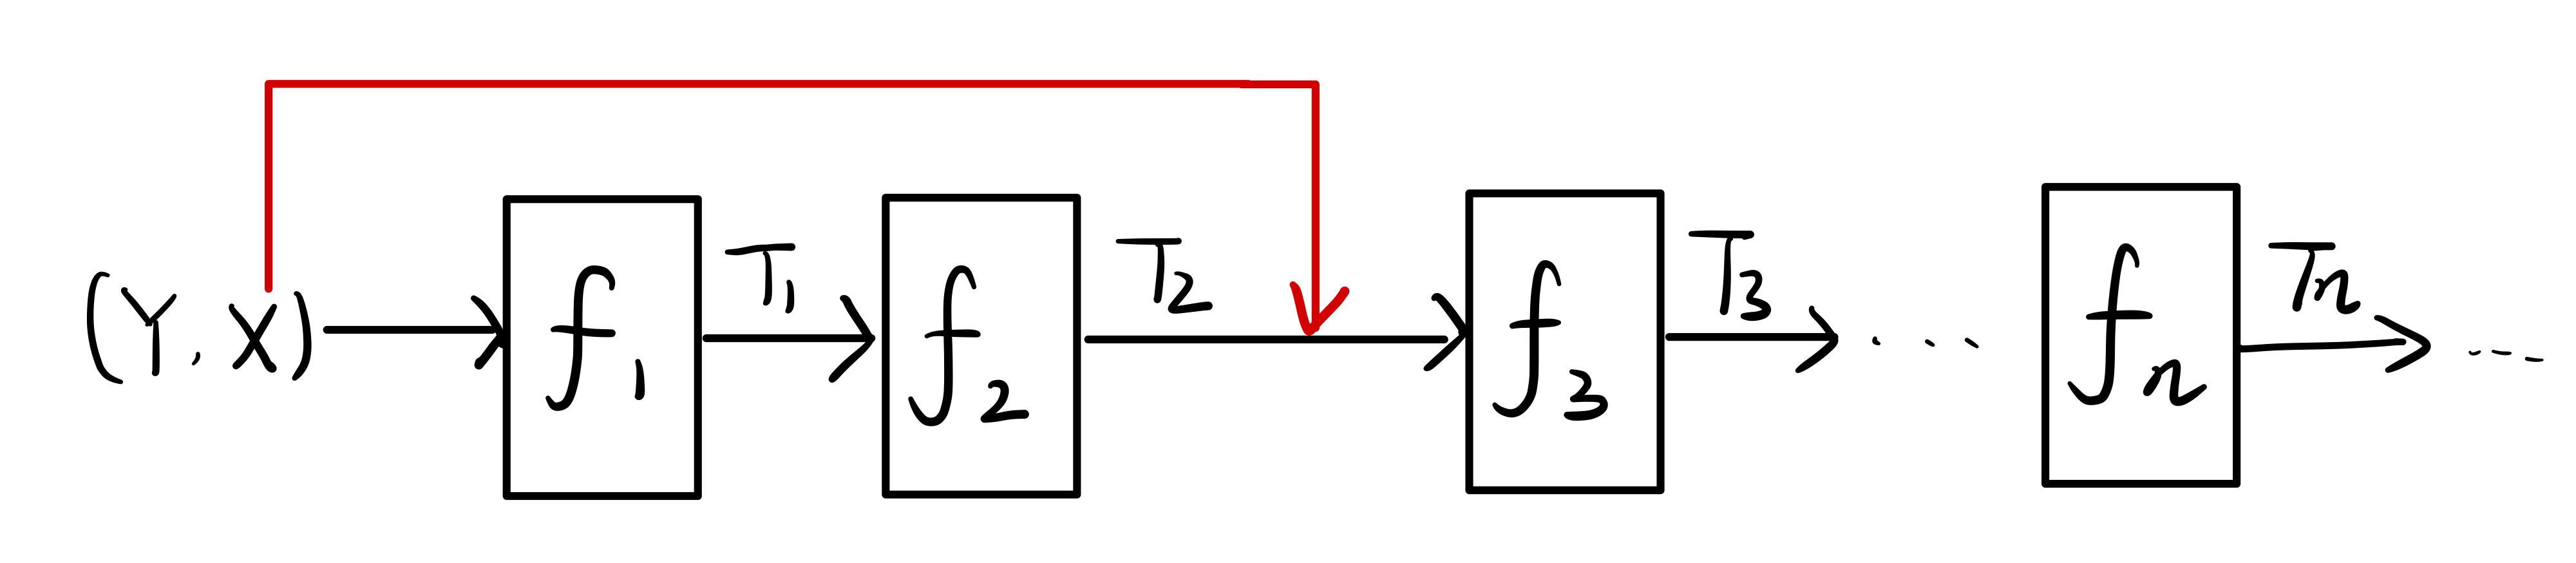
\includegraphics[width=\textwidth]{./figures/chapter1/data_processing.png}
\end{figure}
不加红色的跳层连接: $X\rightarrow T_1\rightarrow T_2\rightarrow\cdots\rightarrow T_n$

加红色的跳层连接: $(X, T_2)\rightarrow T_3\rightarrow\cdots$

在没有保障的情况下, $T_n$ 与 $Y$ 的互信息随$n$的增加不断减少. 为了保障$T_n$与$Y$的互信息: sufficient statistics(充分统计量), 保留足够的信息.

最极端的情况: 保存的信息s.t. $\hat{Y}=Y$, 保留了全部信息.